In the design phase, the original code of the DBT system was analyzed. In order to obtain a system with modules directly related with the source code and to improve its internal structure, the refactoring process was performed over the original DBT system. This section describes the main modifications and the structure of the final system. 


\subsubsection*{CBuffer and CTransBuffer}

\textbf{CCache} and \textbf{TCache} are two atomic subcomponents of the DBT. In the original source code, they are represented in two classes: \texttt{CBuffer} and \texttt{TBuffer}. Since these classes only define services, there was no need for modifications of the source files.

\begin{figure}[H]
\centerline{
\includegraphics[scale=0.5]{images/Refactor_caches}
}
\caption{CBuffer and CTransBuffer UML diagram.}
\label{fig:refactorcaches} 
\end{figure}


\subsubsection*{CSourceArchitecture and C8051Arch}

Since the \textbf{Source Cluster} is one of the main components of the \textit{DBT}, an arrangement in the original source code was made in order to associate its subcomponents: \textbf{Source Architecture}, \textbf{Decoder} and \textbf{SourceEnvironment}. 

Respecting the reference architecture, a base class called \texttt{CSourceArchitecture} was created in order to encapsulate the abstract behavior of the Source Cluster related to all of its subcomponents. The class members were defined accordingly with the interaction presented in the DBT model. Those members are:
\begin{itemize}
\item An object of type \texttt{CBuffer}, which stores source code and has services used by the source cluster components (\textbf{composition} association).
\item An object of type \texttt{SourceEnvironment}, represented in the model as SourceEnvironment component (\textbf{composition} association).
\item A pointer to the class \texttt{CTargetArchitecture}, allowing the subcomponents of the source cluster to reference services provided by the components defined the target cluster (\textbf{aggregation} association).
\item Pointers to internal variables declared in \texttt{CDBTEngine} (explained latter) such as \texttt{eoBB, eoExec} and \texttt{SourcePMem} since those belong to an interface declared as a service in the DBTEngine component.
\item A virtual method called \texttt{decode} with the same role as in the original code.
\end{itemize} 

The base class was created in order to allow the redefinition of a specific source architecture in a easy way. By so, a concrete class named \texttt{C8051Arch} was implemented, which derives from \texttt{CSourceArchitecture} and implements all specific behavior. Thus, the \texttt{decode} method was overloaded (virtual function) and additional methods were added (\texttt{fineDecode0x0, fineDecode0x1}, ...) to perform the decode procedure. Anytime a designer intends to change the source architecture, a similar class must be created and derived from the referred base class. In this way, all interfaces are respected since it inherits all methods and variables.

\begin{figure}[!htb]
\centerline{
\includegraphics[scale=0.53]{images/Refactor_src}
}
\caption{CSourceArchiecture and C8051Arch UML diagram.}
\label{fig:sourcearchitectureUML} 
\end{figure}



\subsubsection*{CTargetArchitecture and CCortexM3}

The idea behind the Source Cluster class representation in the project is the same as the \textbf{Target Cluster}. This components is composed by two components: \textbf{TargetArchitecture} and \textbf{Generator}. A base class was created, called \texttt{CTargetArchitecture}, which has the abstract behavior of the Target Cluster component. This class defines all variables and methods that must be overloaded by a specific target architecture class, in order to respect the interfaces established in the model.  The basic class is composed by the following members:

\begin{itemize}
\item An object of type \texttt{CTransBuffer}, which stores translated code and has methods used by the target cluster components (\textbf{composition} association).
\item A pointer to an object of type \texttt{SourceEnvironment} (\textbf{aggregation} association), since the Generator component references services provided by this class.
\item A pointer to an internal variable of the \texttt{DBTEngine} class, \texttt{eoBB}, referenced also by the Generator.
\item Generic virtual methods (\texttt{gen\_X} functions) used to implement the target code generation. 
\end{itemize}

\begin{figure}[H]
\centerline{
\includegraphics[scale=0.5]{images/Refactor_trg}
}
\caption{CTargetArchitecture and CCortexM3 UML Diagram}
\label{fig:refactortrg} 
\end{figure}


Like \texttt{C8051Arch}, a concrete class for a specific target architecture must be derived from the base class \texttt{CTargetArchitecture}, in order to implement the specific behavior for the generator component. 


\subsubsection*{CDBTEngine}

The final structural modification was done to add another class to the project: \texttt{CDBTEngine}. This class encapsulates the engine of the DBT, namely, the process of translation of source code stored in \texttt{CBuffer} and execution of native code stored in \texttt{CTransBuffer}. 

The class contains the following variables and function members:
\begin{itemize}
\item Two objects of type \texttt{C8051Arch} and \texttt{CCortexM3} (\textbf{composition}), each one providing services from each cluster.
\item Several variables such as \texttt{eoExec, eoBB, SourcePMem, exit\_addr and sourceProgSize}, all used in internally in the engine.
\item A method used for the initialization of the DBT (\texttt{initTranslator}) and another for running (\texttt{runDBT}).
\item Two methods identified as components in the model: \texttt{execute} and \texttt{translate}.
\end{itemize}


\begin{figure}[H]
\centerline{
\includegraphics[scale=0.6]{images/Refactor_DBTEngine}
}
\caption{CDBTEngine UML diagram.}
\label{fig:refactorproject} 
\end{figure}


\subsubsection*{Project Sources and Headers}

Given the fact that new classes were added and others deleted, the organization of the final project sources was different form the original. New source files were added to encapsulate the new classes and new headers were created to have all definitions organized by their type.

Figure \ref{fig:refactorunderstand} shows a dependency graph created using the framework \textit{Understand™}, containing the source files of the DBT organized by subcomponents (\textbf{Target Cluster, Source Cluster, TCache, CCache} and \textbf{DBTEngine}).
 
\begin{figure}[!htb]
\centerline{
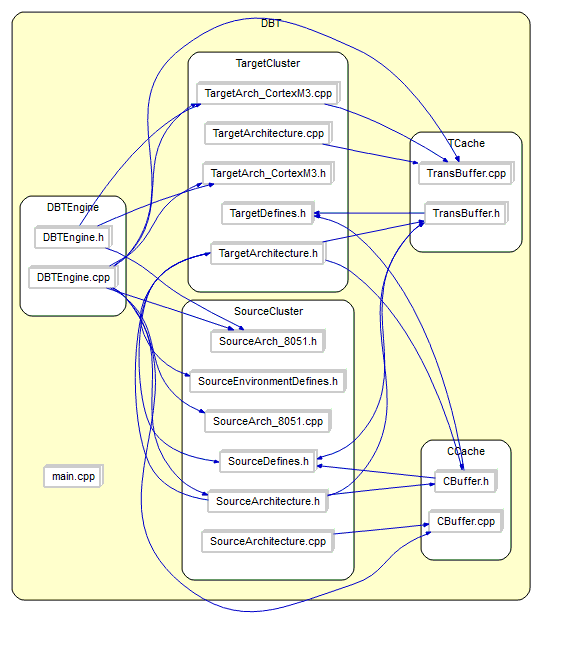
\includegraphics[scale=0.7]{images/DBT_understand}
}
\caption{Dependency graph of the DBT project files.}
\label{fig:refactorunderstand} 
\end{figure}

The dependencies observed were created using \textbf{calls} and \textbf{imports}. It becomes evident the relationship between the code of the project and the model created for the DBT. Comparing figure \ref{fig:refactorunderstand} (new version) with figure \ref{fig:understand} (old version), it is possible to see that:
\begin{itemize}
\item Four files were deleted (\texttt{Translate.cpp, Translate.h, Translate8051.cpp} and \texttt{Translate8051.h}.
\item Six files were added related with the source architecture (\texttt{SourceArchitecture.cpp}, \texttt{SourceArchitecture.h}, \texttt{SourceArch\_8051.cpp}, \texttt{SourceArch\_8051.h}, \texttt{SourceEnvironmentDefines.h} and \texttt{SourceDefines.h}).
\item Five files were added related with the target architecture (\texttt{TargetArchitecture.cpp}, \texttt{TargetArchietcture.h}, \texttt{TargetDefines.h}, \texttt{TargetArch\_CortexM3.cpp} and \texttt{TargetArch\_CortexM3.h}).
\item Two files were added containing the DBT engine (\texttt{DBTEngine.cpp} and \texttt{DBTEngine.h})
\end{itemize}

The referred files contain the classes that were created. However, there are two new headers that are composed by definitions of both architectures: \texttt{SourceDefines.h} and \texttt{TargetDefines.h}. These files are deeply related with the services provided by the architectures components of the model, i.e., the name of the registers, the size of the memories, the size of the word, among others. 